\section{Auswertung}
\label{sec:Auswertung}

Die sowohl für $p \leq \qty{1}{\bar}$, als auch für $p>\qty{1}{\bar}$ aufgenommenen Werte für $T$ und $p$ wurden in \ref{tab:tabelle1} angeführt.
\begin{table}[H]
    \label{tab:tabelle1}
    \begin{tblr}{
        colspec={S[table-format=3.0] S[table-format=1.3]},
        row{1}={guard, mode=math}}
        \toprule
        T \mathbin{/} \unit{\celsius} & p \mathbin{/} \unit{\bar}\\
        \midrule
        19  &   0.057       \\
        20  &   0.076       \\
        21  &   0.081       \\
        22  &   0.086       \\
        23  &   0.090       \\
        24  &   0.094       \\
        25  &   0.098       \\
        26  &   0.102       \\
        27  &   0.105       \\
        28  &   0.109       \\
        29  &   0.113       \\
        30  &   0.116       \\
        31  &   0.120       \\
        32  &   0.124       \\
        33  &   0.127       \\
        34  &   0.131       \\
        35  &   0.135       \\
        36  &   0.138       \\
        37  &   0.143       \\
        38  &   0.146       \\
        39  &   0.150       \\
        40  &   0.154       \\
        41  &   0.157       \\
        42  &   0.161       \\
        43  &   0.165       \\
        44  &   0.170       \\
        45  &   0.175       \\
        46  &   0.179       \\
        47  &   0.184       \\
        48  &   0.189       \\
        49  &   0.194       \\
        50  &   0.197       \\
        51  &   0.204       \\
        52  &   0.210       \\
        53  &   0.215       \\
        54  &   0.221       \\
        55  &   0.226       \\
        56  &   0.231       \\
        57  &   0.238       \\
        58  &   0.246       \\
        59  &   0.251       \\
        60  &   0.257       \\
        61  &   0.263       \\
        62  &   0.268       \\
        63  &   0.278       \\
        64  &   0.285       \\
        65  &   0.293       \\
        66  &   0.301       \\
        67  &   0.311       \\
        68  &   0.320       \\
        69  &   0.328       \\
        70  &   0.340       \\
        71  &   0.349       \\
        72  &   0.361       \\
        73  &   0.373       \\
        74  &   0.386       \\
        75  &   0.400       \\
        76  &   0.416       \\
        77  &   0.434       \\
        78  &   0.450       \\
        79  &   0.469       \\
        80  &   0.488       \\
        81  &   0.505       \\
        82  &   0.524       \\
        83  &   0.545       \\
        84  &   0.564       \\
        85  &   0.587       \\
        86  &   0.605       \\
        87  &   0.627       \\
        88  &   0.641       \\
        89  &   0.656       \\
        90  &   0.676       \\
        91  &   0.701       \\
        92  &   0.734       \\
        93  &   0.759       \\
        94  &   0.782       \\
        95  &   0.806       \\
        96  &   0.832       \\
        97  &   0.861       \\
        98  &   0.890       \\
        99  &   0.914       \\
        100 &   0.947       \\
        101 &   0.955       \\
        102 &   0.958       \\
        103 &   0.962       \\
        104 &   0.968       \\
        105 &   0.970       \\
        109 &   0.971       \\
        110 &   0.971       \\
        111 &   0.974       \\
        112 &   0.974       \\
        113 &   0.974       \\
        118 &   1           \\
        131 &   2           \\
        141 &   3           \\
        149 &   4           \\
        156 &   5           \\
        161 &   6           \\
        167 &   7           \\
        172 &   8           \\
        173 &   9           \\
        181 &  10           \\
        186 &  11           \\
        189 &  12           \\
        192 &  13           \\
        195 &  14           \\
        198 &  15           \\
        \bottomrule
    \end{tblr}
\end{table}

Um einen Mittelwert für die Verdampfungswärme zu bestimmen, wurde die Temperatur in Kelvin umgerechnet und der Kehrwert gebildet.
Für den Druck wurde eine logarithmische Skala gewählt.
Diese Daten wurden in der Abbildung \ref{fig:werte} dargestellt.

\begin{figure}[H]
    \centering
    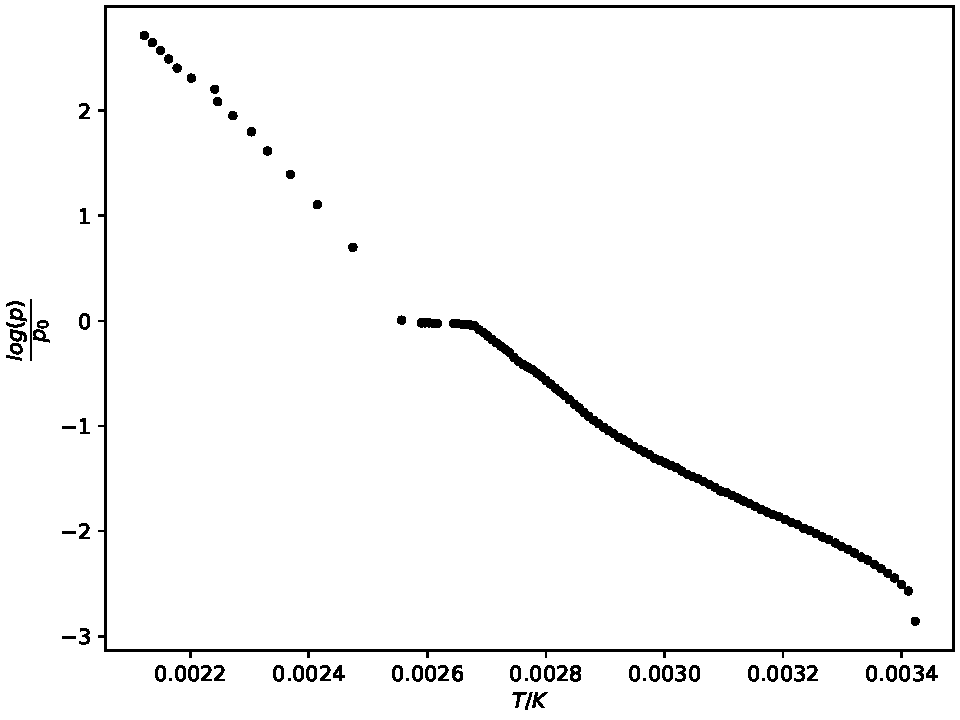
\includegraphics{plot1.pdf}
    \caption{Hier ist der Dampfdruck in Bar auf einer logarithmischen Skala gegen die Temperatur in Kelvin aufgetragen.}
    \label{fig:werte}
\end{figure}

Für den Bereich $p \leq \qty{1}{\bar}$ wurde dann lineare Regression angewandt.
Die in der Abbildung \ref{fig:regression} eingezeichnete Ausgleichsgerade besitzt die Steigung $a=\qty{-3282.759(36.723)}{\joule\per\kilo\gram}$.  
Diese entspricht $T\cdot\ln{\frac{p}{p_0}}$.
Gleichung \ref{eqn:druck} wird nach der Verdampfungswärme umgestellt und die Steigung der Ausgleichsgeraden wird in 
\begin{equation*}
    L=-TR\ln{\fac{p}{p_0}}
\end{equation*}
eingesetzt.
Damit ergibt sich $L=
\begin{figure}[H]
    \centering
    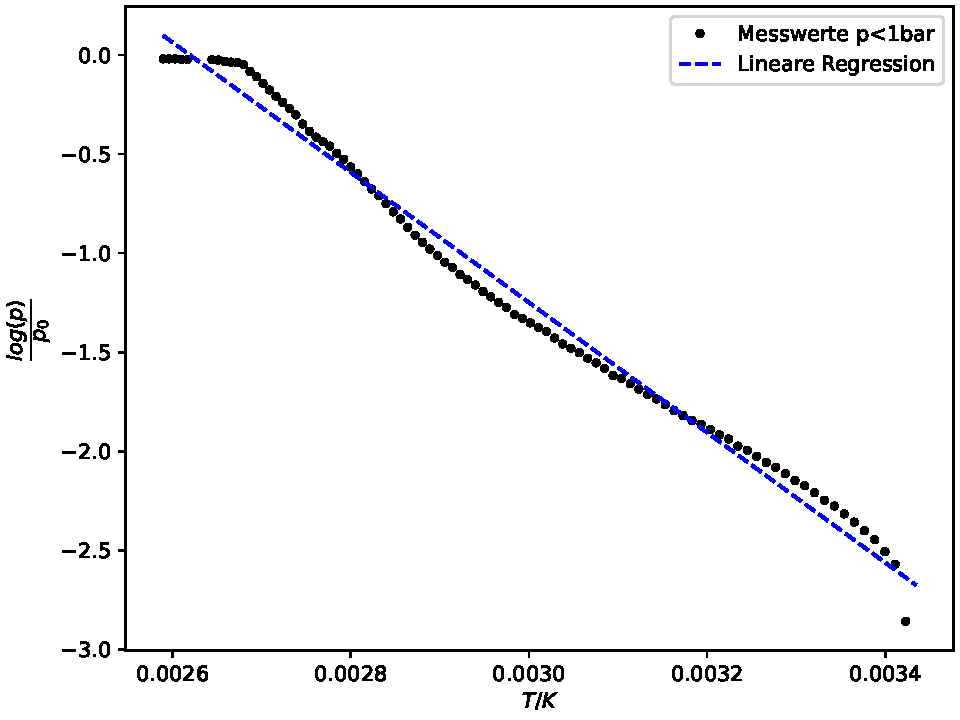
\includegraphics{plot.pdf}
    \caption{Dargestellt ist der Dampfdruck in Bar in logarithmischer Skala, in Abhängigkeit zur Temperatur in Kelvin.
    Zudem wurde eine Ausgleichsgerade eingefügt.}
    \label{fig:regression}
  \end{figure}


